\section{Теоретическое исследование}

\subsection{Расширяемость и автоматизация как единое понятие}
\label{sec:autom-and-ext-as-one-thing}

Во введении были даны определения расширяемости и автоматизации программного обеспечения. С одной стороны, эти два понятия имеют мало общего и могут существовать раздельно. Действительно, программный продукт может предоставлять возможность использовать скрипты для автоматизации, но не поддерживать плагины-расширения. Или наоборот, для приложения может быть разработана развитая система плагинов с автоматическим контролем и обновлением версий, с удобным <<магазином>> расширений, но поддержка автоматизации может отсутствовать.

Как будет показано далее, некоторые существующие решения для интеграции возможностей автоматизации и расширяемости поддерживают сразу оба механизма, некоторые --- только что-то одно. Этому есть объяснение. В некоторых случаях нет необходимости реализовывать оба подхода. Этот вывод подтверждается практикой --- многие современные приложения поддерживают либо автоматизацию, либо расширения, и этого бывает достаточно. Но, как говорилось во введении, данные вопросы встают более остро в крупных программных комплексах, состоящих из множества компонентов. В таких ситуациях зачастую актуальны оба понятия. В связи с этим был сделан вывод о том, что понятия автоматизации и расширяемости можно рассматривать как одно целое. Более того, если это учесть при дизайне приложения, реализовывать поддержку этих механизмов также можно совместно и сделать их неразделимыми.




Для написания пользовательских расширений могут использоваться как скрипты (в терминологии некоторых программ «макросы»)~\cite{automata-via-macros}, так и плагины (независимые модули, написанные на компилируемых языках)~\cite{addins-and-extensibility}.

\subsubsection{Скриптовый язык удобен в следующих случаях:}

\begin{enumerate}
\item Если нужно обеспечить программируемость без риска дестабилизировать систему. Так как, в отличие от плагинов, скрипты интерпретируются, а не компилируются, неправильно написанный скрипт выведет диагностическое сообщение, а не приведёт к системному краху;
\item Если важен выразительный код. Во-первых, чем сложнее система, тем больше кода приходится писать «потому, что это нужно. Во-вторых, в скриптовом языке может быть совсем другая концепция программирования, чем в основной программе — например, игра может быть монолитным однопоточным приложением, в то время как управляющие персонажами скрипты выполняются параллельно. В-третьих, скриптовый язык имеет собственный проблемно-ориентированный набор команд, и одна строка скрипта может делать то же, что несколько десятков строк на традиционном языке. Как следствие, на скриптовом языке может писать программист очень низкой квалификации — например, дизайнер своими руками, не полагаясь на программистов, может корректировать правила игры;
\item Если требуется кроссплатформенность. Хорошим примером является JavaScript — его исполняют браузеры под самыми разными ОС.
\end{enumerate}

\subsubsection{У плагинов же есть три важных преимущества:}

\begin{enumerate}
\item Готовые программы, оттранслированные в машинный код, выполняются значительно быстрее скриптов, которые интерпретируются из исходного кода динамически при каждом исполнении. Поэтому скриптовые языки не применяются для написания программ, требующих оптимальности и быстроты исполнения. Но из-за простоты они часто применяются для написания небольших, одноразовых («проблемных») программ;
\item Полный доступ к любому аппаратному обеспечению или ресурсу ОС (в скриптовом языке для этого должен существовать написанный на машинном коде API). Плагины, работающие с аппаратным обеспечением, традиционно называют драйверами;
\item Если предполагается интенсивный обмен данными между основной программой и пользовательским расширением, для плагина его обеспечить проще.
\end{enumerate}

Также в плане быстродействия скриптовые языки можно разделить на языки динамического разбора (sh) и предварительно компилируемые (perl). Языки динамического разбора считывают инструкции из файла программы минимально требующимися блоками, и исполняют эти блоки, не читая дальнейший код. Предкомпилируемые языки транслируют всю программу в байт-код и затем исполняют его. Некоторые скриптовые языки имеют возможность компиляции программы «на лету» в машинный код (т. н. JIT-компиляция).
\subsection{Применимость существующих решений}
\paragraph{VBA}
\paragraph{VSTA}
\paragraph{VSTO}


\subsection{Задачи, подлежащие решению}

На основании обзора существующих программных продуктов для решения первоначально поставленной задачи и попытке использования {\it Microsoft VSTA}~\cite{vsta-website} (см. главу \ref{sec:use_exis_techn}), было принято решения разрабатывать собственную платформу, в основе которой будет идея реализации единого механизма для поддержки плагинов и скриптов. В данном случае, понятие <<поддержка>> включает в себя средства разработки, механизм взаимодействия с приложением, <<глубина интеграции>> в приложение, а так же механизмы хранения и распространения расширений. Безусловно, основная цель работы, сформулированная в главе \ref{sec:problem_statement}, остается неизменной.

\subsubsection{Основные требования к программному продукту}

Согласно сценариям использования приложения, рассмотренным в главе \ref{sec:pl_requirements}, можно сформулировать основные требования к платформе поддержки расширений и скриптов. Среди них есть так и обязательные, так и опциональные, реализация которых желательна, но в рамках решения текущей задачи может и не быть выполнена. Однако, описанные возможности могут быть добавлены в платформу во время дальнейшего развития работы.

{\bf Обязательные требования:}

\label{sec:requirements}
\begin{enumerate}
	\item Возможность создания расширений для конечных пользователей;
	\item Простота использования (Не требует SDK и другого ПО для создания расширений. Вся работа происходит в среде разработки (IDE));
	\item Возможность работы как под x86, так и под x64 архитектурами;
	\item Возможность отладки расширения;
	\item Доступ расширения к объектам расширяемого приложения, реакция на его события;
	\item При изменении удалении или добавлении объекта в хост приложении, расширение должно автоматически обновлять информацию о своем окружении;
	\item Доступ к библиотеке классов .NET Framework;
	\item Поддержка большого числа расширений, работающих одновременно;
	\item Удобные инструменты для написания кода (Аналогично инструментам IntelliSense в Microsoft Visual Studio);
	\item Возможность сохранения расширений по усмотрению пользователя в базу данных, архив, папку и т. д.;
	\item Динамическая загрузка и выгрузка расширений из адресного пространства хост приложения;
	\item Компиляция и перезагрузка расширения «на лету» (Не требуется перезапуск хост приложения).
\end{enumerate}

{\bf Опциональные требования:}
\label{sec:opt_requirements}
\begin{enumerate}
	\item Реализация взаимодействия расширений друг с другом;
	\item Возможность разрешения зависимостей между расширениями;
	\item Возможность записи последовательности действий пользователя в виде макроса;
	\item Реализация средств для облегчения внедрения платформы (Анализ кода расширяемого приложения, автоматическая генерация прокси-объектов);
	\item Централизованное распространение расширений при помощи репозитория.
\end{enumerate}

\subsubsection{Список задач}

Исходя из сформулированных выше требований можно произвести декомпозицию основной цели <<реализация рлатформы>> на ряд задач.

\begin{enumerate}
	\item Интеграция со средой разработки;
	\item Межпроцессное взаимодействие;
	\item Взаимодействие расширений с приложением;
	\item Интеграция платформы в расширяемое приложение.
\end{enumerate}

Методы решения этих задач будут подробно рассмотрены далее.

%\section{Разработка платформы}

Ранее (см. раздел~\ref{sec:requirements}) уже были сформулированы основные требования к разрабатываемой платформе. При проектировании архитектуры платформы должны учитываться эти требования, преимущества и недостатки рассмотренных существующих решений, а также опыт внедрения одного из таких решений на реальном проекте (см. раздел~\ref{sec:use-itm-vsta}).

Вполне логично разделить систему на два компонента:
\begin{itemize}
 \item интерактивная среда разработки, содержащая в себе текстовый редактор, средство для управления проектами, отладчик и прочие дополнительные инструменты, упрощающие процесс разработки скриптов. Этому вопросу посвящён раздел~\ref{sec:ide-integration};
 \item модуль, встраиваемый в основное (расширяемое) приложение.
\end{itemize}

Такое глобальное разделение системы на две части даёт следующие преимущества:
\begin{enumerate}
 \item Независимость компонентов. Если возникнет необходимость заменить используемую среду разработки на другую, этого можно будет достичь, минимально меняя второй компонент системы;
 \item Стабильность. В случае аварийного завершения (или каких-либо ошибок) внутри среды разработки работа основного приложения с большей долей вероятности не будет затронута;
 \item Безопасность. Доступ к данным основного приложения строго определяется протоколом взаимодействия компонентов системы.
\end{enumerate}

Описанные компоненты системы выполняются в разных процессах. Это добавляет им независимости. Помимо этого, забегая вперёд, отметим, что это позволит проще реализовать отладку. Таким образом, нужно выбрать способ межпроцессного взаимодействия, который позволит максимально просто и эффективно взаимодействовать компонентам системы. Этому вопросу посвящен раздел~\ref{sec:ipc}.

\subsection{Интеграция со средой разработки}

Один из важнейших сценариев использования расширяемых и автоматизируемых программных продуктов --- возможность разработки новых скриптов и редактирование кода старых в интегрированной среде разработки.

Встроенная среда разработки как правило поставляется вместе с продуктами для автоматизации приложений, например VBA или VSTA. В платформах, основная цель которых --- поддержка плагинов, напротив, встроенных средств для редактирования кода не предоставляется. Это понятно, так как считается, что конечный пользователь не будет заниматься такой сложной задачей, как написание расширения к своему приложению. Для разработчиков же существуют отдельные пакеты (SDK) для разработки расширений в различных средах разработки.

При реализации платформы для автоматизации и расширения необходимо было предоставить удобные средства редактирования кода конечному пользователю. Эта задача может быть решена несколькими способами:

\subsubsection{Реализация собственного редактора исходного кода расширений}

Это решение имеет как и преимущества, так и целый ряд существенных недостатков. Положительным моментом этого подхода является простота интеграции в разрабатываемую платфому. Однако, реализация действительно удобного набора инструментов, таких как подсветка синтаксиса, автодополнение, автогенерация кода по шаблонам, управления файлами с исходным кодом, будет очень сложной задачей. Кроме того, результат в любом случае наврядли сравниться с современными IDE.

\subsubsection{Использование одной из существующих IDE}

Это решение хорошо тем, что мы получаем готовую среду разработки с множеством встроенных инструментов. Одноко, встает ряд вопросов, которые необходимо решить для успешного применения сторонней IDE в разрабатываемой платформе.

Интеграция в платформу. Под интеграцией необходимо понимать возможность программного управления сторонней IDE на уровне, достаточном для того, чтобы у пользователя складывалось ощущение, что он работает с единой системой, а не несколькими разными программами.

Большинство IDE обладают куда более широким, чем нужно для разработки расширений, функционалом. Поэтому важным критерием выбора сторонней IDE является ее настраиваемость и конфигурируемость. Это касается как доступных пользователю функций, так и внешного вида самой среды.

Несмотря на предыдущий пункт, в котором сказано, что функционал современных сред разработки излишен для использования их в качастве редактора расширений, может случиться так, что некоторых специфичных функций будет нехватать. Поэтому искомая среда должна также обладать возможностью расширения функционала. Отдельным плюсом будет поддержка плагинов. Тогда можно будет отключать ненужные плагины и разработать плагины, добавляющие новый функционал.

Рассмотрим существующие среды разработки под платформу .NET.

\subsubsection{MS Visual Studio}

Удобная и мощная среда разработки от компании Microsoft. Распространяется в нескольких редакциях, различных по стоимости и функционалу. Помимо платных Professional и Ultimate версий существует бесплатная Express редакция.

Эта IDE поддерживает плагины, и имеет огромное количество разнообразных расширений, повышающих эффективность разработки.

Так же она поддерживает довольно гибкий механихм пользовательских настроек, что позволяет разработчику настроить ее <<под себя>>. Однако, отключить ненужные функции этот механизм не позволяет.

Поддерживает программное управление благодаря наличию  DTE --- объекта верхнего уровня в объектной модели автоматизации Visual Studio. Этот объект используется для доступа к функциональности. Доступ к этому объекту осуществляется через EnvDTE — это обернутая сборка COM-библиотеки, содержащая объекты и члены для автоматизации ядра Visual Studio. При помощи DTE можно программно управлять средой разработки, переопределять ее поведение. Таким образом Visual Studio может быть интегрирована в платформу.

Стоит отметить, что использование DTE для управления бесплатной версией Visual Studio Express невозможно, так как в ней отсутствуют необходимые для этого компоненты.

\subsubsection{SharpDevelop}

SharpDevelop — свободная среда разработки для C\#, Visual Basic .NET, Boo, IronPython, IronRuby, F\#, C++. Обычно используется теми, кто не хочет пользоваться Visual Studio .NET.

SharpDevelop предоставляет интегрированный отладчик, который использует собственные библиотеки и взаимодействует с исполняющей средой .NET через COM Interop.

У этой среды разработки есть ряд особенностей и преимуществ:

Во-первых, эта IDE может управляться программно извне при помощи встроенной технологии SDA (SharpDevelop for Applications). Программное управление позволяет выполнять различные действия в IDE без участия пользователя. Например, показывать или скрывать само приложение, запускать сборку проекта, управлять сохранением и загрузкой проектов, и многие другие. 

Во-вторых, эта IDE поддерживает плагины. Это свойство позволит добавить какую-либо отсутствующую в базовой поставке функциональность не меняя исходного кода самого SharpDevelop. Это важно, так как изменение исходного кода сделает неудобным распространение готовой платформы, так как она будет совместима только с конкретной сборкой SharpDevelop. Использование плагинов позволит добавить нужную функцинальность в уже установленный экземпляр этой IDE.

В-третьих, SharpDevelop поддерживает кастомизацию, то есть изменение своего внешного вида и поведения при момощи конфигурационных файлов. Под изменением внешнего вида нужно понимать удаление <<лишних>> в контексте данного сценария использования (как внешней IDE для разработки расширений) элементов управления, добавление новых элементов управления, управление доступностью этих элементов, и прочее. Изменение поведения состоит в подмене штатных обработчиков событий элементов управления (например, кнопок), на свои собственные обработчики с измененной логикой. Например, запуск отладчика не должен пытаться стартовать сборку самого расширения (это попросту невозможно, так как расширения представляет из себя библиотеку классов), а присоединить отладчик к процессу хост-приложения.

В-четвертых, открытый исходных код поможет быстрее решить проблемы, связанные с интеграцией SharpDevelop в разрабатываемую платформу. Код IDE может быть отредактирован благодаря открытой лиценции GNU GPL v2. IDE может быть запущена под отладчиком для выявления и локализации проблем вызванных внешними факторами и нетипичным использованием самой IDE.

Наконец, она распространяется бесплатно, что делает ее очень привлекательным выбором для использования в разрабатываемой платформе.

Из недостатков этой среды стоит отметить не такой богатый инструментарий, как в VisualStudio, отсутствие аналогов многих полулярных в сообществе .NET-разработчиков в среде  VisualStudio планинов, таких как ReSharper. Не такой удобный редактор исходного кода и визуальных элементов. С другой стороны, SharpDevelop не такой <<тяжеловесный>> и потребляет мало ресурсов, что немаловажный фактор в предполагаемом сценарии его использования, как внешней среды для редактирования исходного кода расширений.

\subsubsection{MonoDevelop}

Этот продукт является кроссплатформенным форком, то есть клоном SharpDevelop, и имеет сходный с ним функционал. Более подробно рассматривать ее не имеет большого смысла. Все плюсы и минусы SharpDevelop имеют отношение и к MonoDevelop. Однако, MonoDevelop не поддерживает программное управление, в отличие от SharpDevelop, что делает SharpDevelop более предпочтительным выбором для решения поставленной задачи.

\subsubsection{Вывод}

В качестве внешней IDE для разработки расширений была выбрана IDE с открытым исходным кодом SharpDevelop. Помимо того, что она распространяется бесплатно, имеет открытый исходный код и потребляет меньше ресурсов системы под свои нужды, инсталляционный пакет SharpDevelop имеет куда меньшие размеры, чем Visual Studio, и не содержит такое многообразие различных компонент, которые будут лишними на рабочей станции рядового пользователя ПО (не разработчика).

\pagebreak

\subsection{Межпроцессное взаимодействие}
\label{sec:ipc}

В каждой операционной системе предоставляются различные способы межпроцессного взаимодействия. Ниже перечислены наиболее популярные из них:
\begin{itemize}
   \item использование доступа к общему файлу;
   \item использование сигналов;
   \item сокеты;
   \item именованные каналы;
   \item разделяемая память;
   \item очереди сообщений.
\end{itemize}

Некоторые способы можно реализовывать вручную, для некоторых есть специальные функции в API операционной системы. Однако более высокоуровневые библиотеки и платформы, такие как {\it .NET}, предоставляют обобщённые и более универсальные механизмы для межпроцессного взаимодействия. Ниже будет рассмотрен один из них.

{\it WCF (Windows Communication Foundation)} --- программный фреймворк, используемый для обмена данными между приложениями, входящими в состав {\it .NET Framework}~\cite{wcf-unleashed}. {\it WCF} делает возможным построение безопасных и надёжных транзакционных систем через упрощённую унифицированную программную модель межплатформенного взаимодействия. Если не вдаваться в подробности, можно сказать, что {\it WCF} --- некая абстракция, обёртка, которая скрывает фактические детали реализации межпроцессного взаимодействия, которое на низком уровне будет реализовано за счёт одного из вышеперечисленных способов. 

Для осуществления межпроцессного взаимодействия должен быть написан интерфейс, который будет реализован в одном из процессов. Процесс, реализующий интерфейс, предоставляет сервис (службу), к которой может подключиться другой процесс, удалённо вызывая методы интерфейса~\cite{wcf-services}. Для обратного взаимодействия можно использовать callback-вызовы, либо создавать и реализовывать ещё один интерфейс и открывать второй канал для взаимодействия в обратную сторону. 

В разрабатываемой платформе межпроцессное взаимодействие нужно для:
\begin{itemize}
 \item управления средой разработки;
 \item передачи дополнительных данных среде разработки;
 \item передачи событий среды основному приложению.
\end{itemize}


\pagebreak

\subsection{Интеграция расширений}
\label{sec:extention_interaction}

\TODO{обзор возможных технологий, выводы}

\pagebreak

\subsection{Интеграция в расширяемое приложение}
\label{sec:app-integration}

Задачу интеграции разрабатываемой платформы можно разделить на два случая:

\begin{itemize}
  \item интеграция в готовое приложение;
  \item интеграция в приложение на этапе разработки.
\end{itemize}

Задача интеграции платформы в разрабатывоемое приложение не вызывает затруднений как для платформы, описываемой в работе, так и для большинства рассмотреных аналогов, так как на этом этапе программист имеет возможность продумать архитектуру приложения с учетом использования того или иного решения для интеграции возможностей автоматизации и/или расширения. Сложность интеграции в этом случае в большей степени зависит от решений, принятых разработчиком, чем от принципов, заложенных в интегрируемом продукте. Безусловно, лубой продукт требует наличия опыта работы с ним для получения лучших результатов.

Куда более интересна задача интеграции платформы в приложение, код которого уже написан, и архитектура не потерпит изменений. В этом случае большинство из существующих решений оказывабтся настолько сложны в интеграции из-за особенностей своего внутреннего устройства, что можно заявлять, что для этих продуктов такая задача будет практически неразрешимой. Все дело в сложности принципов построения взаимодействия между расширением и приложением, заложенных в большинстве существующих решений. Эти принципы сложны, потому что преследуют цели полной изоляции приложения от расширения, создания универсальных механизмов взаимодействия, а так же из-за использования тех или иных шаблонов проектирования. Этот факт не делает существующие решения плохими, наоборот, все решения, используемые в этих продуктах имеют серьёзное теоретическое обоснование, диктуемое принципапи проектирования программного обеспечения, но, к сожалению, из-за этого применение существующих решений в рамках интеграции возможностей расширения в существующее приложение становиться очень трудоёмкой задачей.

В работе стояла именно задача интеграции разрабатываемой платформы в уже существующее приложение. Опираясь на результаты, полученные в предыдущих разделах, решение этой задаци состоит из нескольких этапов:

\begin{itemize}
  \item выделение в коде приложения типов, объекты которых должны быть доступны со стороны расширения;
  \item реализация этими классами интерфейса, предаставляемого модулем платформы, отвечающим за взаимодействие с расширениями;
  \item создание классов-наблюдателей, храшящих список объектов одного типа, и реагирующих на все изменения количества и состояния этих объектов;
  \item регистрация этих классов-наблюдателей в модуле поддержки взаимодействия с расширениями;
  \item внедрение пользовательских элементов управления расширениями, предоставляемых платформой.
\end{itemize}

\pagebreak

%\subsection{Архитектура платформы}
\label{sec:fw_arch}

В этом разделе будет рассмотрена укрупненная схема архитектуры платформы; расположение и назначение компонентов системы и их взаимодействие.

После определения спектра глобальных задач, подлежащих решению в рамках реализации платформы, и выбора используемых для их решения технологий, инструментов и подходов, а также учитывая опыт существующих разработок, направленных на решение поставленной задачи, в особенности {\it VBA} и {\it VSTA}, была разработана концептуальная модель взаимодействия основных компонентов платформы~\cite{patterns-of-enterprise-app}.

Как видно на рисунке \ref{fw_arch1}, система состоит из двух отдельных процессов. Такая архитектура обусловлена необходимостью поддержку отладки расширений, а отладчик, как известно, должен выполняться в отдельном процессе. Кроме того, хост-процесс IDE является дочерним для процесса хост-приложения. Управление этими процессами организовано таким образом, что в случае прекращения из-за критической ошибки работы процесса, обслуживающего IDE, этот процесс будет автоматически перезапущен. В таком случае система продолжит работу в штатном режиме. Напротив, при сбое в процессе хост-приложения, будет остановлен так же хост-процесс IDE, что позволяет предотвратить возникновения в системе <<паразитных>> процессов.

Согласно разделу \ref{sec:ide-integration}, в качестве внешней среду разработки была выбрана свободная среда разработки с открытым исходным кодом SharpDevelop. Более того, благодаря совместимости библиотек входящих в состав этой IDE, реализована поддержка версий SharpDevelop 3.2 и 4.1, а так же не исключается возможность поддержки последующих версий. Таким образом, реализуемая платформа может быть с успехом использована в приложениях, реализованных на различных версиях платформы .NET. Для временного хранения managed-сборок расширений, компилируемых средой разработки, используется изолированное хранилище. Подробнее про управление сборками расширений написано в разделе \ref{sec:dll_manip}.

\begin{figure}[!h]
    \centering
    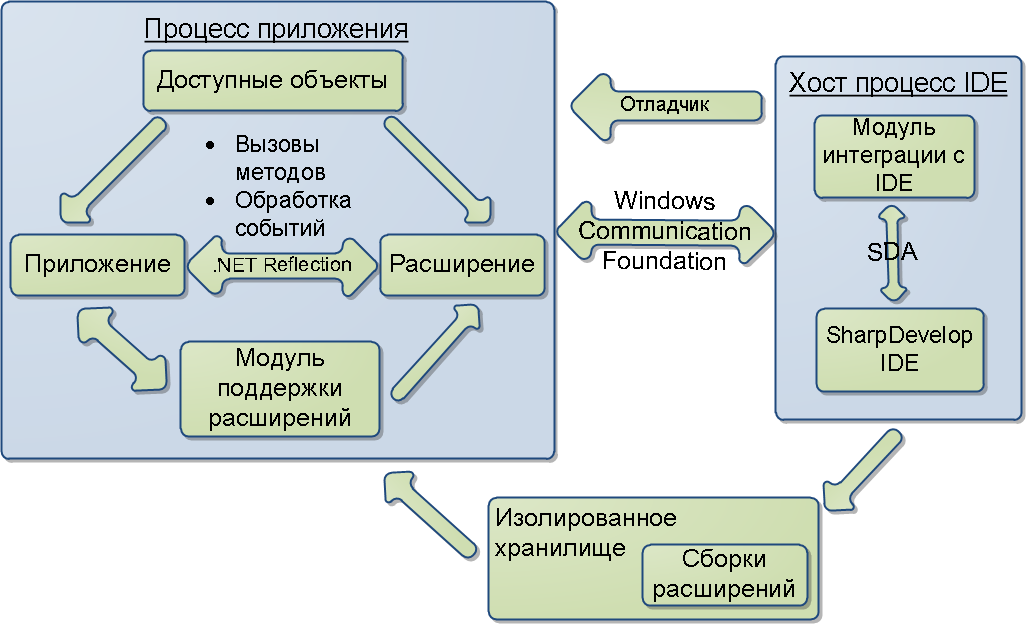
\includegraphics[width=15cm]{fw_arch1_fixed.png}
    \caption{Взаимодействие компонентов системы}
    \label{fw_arch1}
\end{figure}

Межпроцессное взаимодействие в разрабатываемой системе было решено реализовать при помощи именованных каналов {\tt (named pipe)} из библиотеки WCF (Windows Communication Foundation)~\cite{wcf-services}. Выбор WCF обусловлен тем, что эта библиотека входит в состав .NET Framework, и использование ее будет наиболее оправдано для разработки приложения под эту платформу. Реализация именнованых каналов в WCF --- NetNamedPipe, выбрана по причине того, что в рамках решения задачи по обеспечению взаимодействия двух процессов на локальной машине нет необходимости в использовании более сложных и емких механизмов взаимодействия, чем именованные каналы. Подробнее особенности реализации межпроцессного взаимодействия были рассмотрены ранее в разделе~\ref{sec:ipc}.

Взаимодействие между процессами происходит по двум отдельным именованным каналам, так как инициировать запросы (то есть выступать в роли сервера) могут оба процесса, и механизм <<запрос --- ответ>> в данном случае не подходит.

Более того, адреса, по которым взаимодействуют процессы выбираются случайно, что позволяет без возникновения конфликтов запускать множество пар процессов <<приложение --- IDE>>. Такое решение позволит использовать разрабатываемую платформу в нескольких приложениях одновременно.

Для работы с расширениями и IDE в приложение должен быть интегрирован специальный модуль, выполняющий сервисные задачи по обеспечению взаимодействия расширения с приложением, приложения с хост-процессом IDE, а так же предоставляющий пользователю набор визуальных компонент для управления системой. Этот модуль показан на рисунке \ref{fw_arch1} (Модуль поддержки расширений). Его назначение и особенности разработки будут описаны далее.

Взаимодействие расширения и приложения реализовано через {\it .NET Reflection}~\cite{cs2008-dotnet35}, как описано в разделе~\ref{sec:extention_interaction}. Взаимодействие осуществляется через динамическое привязывание к доступным объектам приложения, которые должны подчиняться определенным <<правилам игры>>, чтобы быть доступными для расширения. Выделение видимых объектов и создание уровня доступа к ним --- главная задача интеграции платформы в готовое приложение. Подробнее особенности интеграции разрабатываемой платформы были рассмотрены в разделе~\ref{sec:app-integration}.

\pagebreak


\pagebreak